\documentclass[11pt]{article}
% arxiv pdflatex detection
\pdfoutput=1

\usepackage{deauthor}
\usepackage{times}
\usepackage{wrapfig}
\usepackage{graphicx}
\usepackage{xspace}
% \usepackage[it,small]{caption}
% \usepackage[export]{adjustbox}
\usepackage{cite}
\usepackage{amsmath,amssymb,amsfonts}
\usepackage{textcomp}
\usepackage{graphicx}
\usepackage{algorithm}
\usepackage{algorithmic}
\usepackage{xcolor}


% ensure times
\usepackage{txfonts}
\usepackage{url}

\usepackage{balance}  % for  \balance command ON LAST PAGE  (only there!)
\usepackage{booktabs} % For formal tables
\usepackage{enumitem}
\usepackage{multirow}
\usepackage{subcaption}

% \usepackage[pdfpagelabels=false]{hyperref}

\usepackage{listings}

\usepackage{outlines}
\usepackage{authblk}


% Note-related commands.
\usepackage{etoolbox, totcount}
\newtoggle{shownotes}
\toggletrue{shownotes}
\newtotcounter{numnotes}
\newcommand{\note}[3]{
  \iftoggle{shownotes}{\stepcounter{numnotes}\textcolor{#1}{#2: #3}}{}
}

\newtoggle{showusernotes}
% \toggletrue{showusernote}
\newcommand{\joey}[1]{
    \iftoggle{showusernotes}{\note{cyan}{joey}{#1}}{}
}
\newcommand{\gabe}[1]{
    \iftoggle{showusernotes}{\note{magenta}{gabe}{#1}}{}
}
\newcommand{\shankari}[1]{
    \iftoggle{showusernotes}{\note{purple}{shankari}{#1}}{}
}
% Break URLs properly
\def\UrlBreaks{\do-\do\.\do\@\do\\\do\!\do\_\do\|\do\;\do\>\do\]\do\)\do\,\do\?\do\'\do+\do\=\do\#}
\def\UrlBigBreaks{\do\:\do\/}


\title{CoVista: A Unified View on Privacy Sensitive Mobile Contact Tracing Effort}
% \author{Junli Liu}
% % \affil{Integrative Cell Biology Laboratory, School of Biological and Biomedical Sciences,
%   % The Bio physical Sciences Institute, Durham University, Durham, UK}
%
% \author{James Rowe}
% \author{Keith Lindsey}
% % \affil{Some other laboratory, Elsewhere}
% % \author{foo bar}
% % \author{baz boo}
% % \afil

\author{David Culler, Prabal Dutta, Gabe Fierro, Joseph E. Gonzalez, Nathan Pemberton, \\
Johann Schleier-Smith, K. Shankari, Alvin Wan, Thomas Zachariah \\
{\small \texttt{\{culler, prabal, gt.fierro, jegonzal, nathanp\}@berkeley.edu}}\\
{\small \texttt{\{jssmith, shankari, alvinwan, tzachari\}@berkeley.edu}}\\
UC Berkeley
}


% \author{Gabe Fierro}
% \author{Joseph E. Gonzalez}
% \author{Nathan Pemberton}
% \author{Johann Schleier-Smith}
% \author{K. Shankari}
% \author{Alvin Wan}
% \author{Thomas Zachariah}
% \affil{UC Berkeley}

\begin{document}

\maketitle

\begin{abstract}
Governments around the world have become increasingly frustrated with tech giants dictating public health policy. The software created by Apple and Google enables individuals to track their own potential exposure through collated exposure notifications. However, the same software prohibits location tracking, denying key information needed by public health officials for robust contract tracing. This information is needed to treat and isolate COVID-19 positive people, identify transmission hotspots, and protect against continued spread of infection.
In this article, we present two simple ideas: the \textbf{lighthouse} and the \textbf{covid-commons} that address the needs of public health authorities while preserving the privacy-sensitive goals of the Apple and google exposure notification protocols. 
\end{abstract}

\section{Introduction}  
\label{s:intro}
The past decade has observed a surge in the design and deployment of 
decentralized systems. A key reason for this surge is the growing desire in 
the society to have self-governing democratic financial systems that are not 
under the control of a privileged set of entities. A central control often 
translates to a forced trust model with limited provision to support 
transparency and accountability. The adoption of Blockchain, for example, 
is a by-product of the ability to break away from the forced-central control 
in a trust-worthy fashion~\cite{blockchain-book}. The emerging blockchain 
platforms facilitate a reliable execution of any digital contracts 
(i.e., transactions) in a decentralized manner despite the existence of malicious 
actors. At the core of any blockchain platform is a Byzantine 
fault-tolerant (\BFT{}) consensus protocol and a tamper-proof replicated 
ledger~\cite{bedrock,blockchain-book,scalable-ledger}. The \BFT{} 
protocol helps to achieve {\em consensus} on the order of incoming client 
requests among all the replicas, while the ledger logs this agreement. 

Traditional \BFT{} protocols expect a {\em permissioned} system where the 
identities of all the replicas (i.e., participants) are known prior to any 
consensus as they rely on having a verifiable voting right in a democratic 
setting. These protocols rely on a {\em communication-oriented} consensus 
model, where all the participants exchange endorsements across multiple 
rounds before they can reach a decision~\cite{sharper,pbftj,ahl,poe,rcc,geobft,flexitrust,ringbft,mirbft,basil,hotstuff}.
In these protocols, a system of $\n{}$ replicas can reach a common decision 
if at most $\f{}$ of them are malicious, such that $\n{} \ge 3\f{}+1$. 
The $\n{}$ parties are said to reach a decision when at least a majority 
of honest parties agrees to that decision. This decision is logged by 
requiring all the agreeing parties to {\em sign} the decision. Hence, the 
reached decision is considered {\em tamper-proof} because it has support 
of a majority of honest participants.

Despite being around for more than two decades, traditional \BFT{} protocols 
did not see any major practical applications until the introduction of 
blockchain technology. We attribute {\em two} key factors for this lack of 
adoption. (i) To ensure that the malicious participants do not spawn multiple 
identities, these \BFT{} protocols need an authority (i.e., {\em a forced 
trust gateway}) to verify and register every participant to verify every 
vote~\cite{sybil-attack}; some participants may find this intrusive if they 
do not want to reveal their personal information. (ii) To overwrite the ledger, 
malicious participants just require access to the private keys of honest 
participants. In a sense, the proof of the validity of the ledger is not 
self-contained, and it operates on the assumption that the private-keys 
are kept safe externally indefinitely.

To resolve these challenges, initial blockchain platforms such as 
Bitcoin~\cite{bitcoin} and Ethereum~\cite{ether} offer a {\em permissionless} 
model of consensus. These systems employ the {\em Proof-of-Work} (\PoW{}) 
protocol~\cite{bitcoin,ether}, which follows a {\em computation-oriented} 
consensus model and requires all the participants to compete with each other 
and try to solve a complex puzzle. Whichever participant solves the puzzle 
first gets to add a new entry ({\em block}) to the ledger. As a result, 
\PoW{} protocol eliminates the three challenges seen by traditional \BFT{} 
protocols. (i) Malicious participants can spawn multiple identities, but what 
actually matters is the available compute power. (ii) Each block includes 
the hash of the previous block; overwriting the ledger requires recomputing 
all the blocks making it computationally infeasible. (iii) Since reaching the 
consensus is based on presenting the proof of work that is embedded on the 
ledger (i.e., self-contained), there is no longer any need for external 
safe-keeping of private keys to sign endorsements.

These properties offered by \PoW{} protocol help blockchain platforms to 
design a {\em decentralized economy}, where any person can participate in the 
consensus process, and the economy has a self-generating currency to monetize 
its participants. Monetizing the participants is necessary as the \PoW{} 
protocol expects the participants to spend their resources to solve a complex 
puzzle. Clients of the Bitcoin platform, create transactions that exchange 
Bitcoins and send them to the participants (miners) in the \PoW{} protocol. 
These miners check if the transaction is valid; the client has sufficient 
Bitcoins to transfer. If the transaction is valid, they run \PoW{} protocol to include 
this transaction in the ledger. The winning miner of \PoW{} gets a portion of 
the client's Bitcoin as {\em fees}, while the mining process (\PoW{}) mints  
new tokens to fund the economy. This new token is transferred to the winning 
miner's account and is recorded as a transaction in the block.

The key challenge with platforms like Bitcoin is their {\em practicality}. 
These platforms have abysmally low throughput in the order of $10$ transactions 
per second in part due to inadequate choice of small block sizes. Furthermore, as 
more miners join the network, the complexity of the puzzle has to be increased. 
For example, the complexity of the current Bitcoin puzzle is so high that the 
miners work in large groups to have any positive probability of creating the 
next winning block~\cite{blockchain-book}. Moreover, as miners are competing 
with each other, it leads to massive wastage of computational resources (energy) 
as only the winning miner's efforts are recorded and rewarded. This results in an unsustainable ecosystem~\cite{badcoin,badbadcoin}.

We observe these challenges in the designs of existing \BFT{} protocols and 
blockchain platforms and envision a \DualChain{} system that learns from these 
models and eliminates their key challenges. Essentially, we aim to establish a 
new research agenda; a new field of hybrid consensus protocols that depart from 
competitive consensus to a collaborative consensus that is both resilient and 
sustainable. Our \DualChain{} architecture takes a step in this direction by 
running two consensuses on each client transaction while ensuring there is no 
increase in the latency observed by the client. Each client request is first 
ordered through a state-of-the-art \BFT{} consensus protocol ({\em commitment}), 
subsequently, this ordered request is engraved into the ledger through the 
\PoW-style consensus ({\em settlement}). Specifically, \DualChain{} causes no 
increase in commitment latency while improving the settlement latency observed 
by existing protocols. Ordering the client transaction through a \BFT{} consensus 
protocol first allows our \DualChain{} system to guarantee the following benefits: 
(i) clients receive low-latency responses, and (ii) \PoW{} participants no longer 
need to compete, resulting in a high-throughput sustainable chain. As a result, 
instead of employing the \PoW{} for consensus, we design a novel protocol that 
allows miners to collaborate. We refer to this paradigm as 
{\em Power-of-Collaboration} (\PoC{}). 

Our \PoC{} protocol splits the complex puzzle into disjoint slices and requires 
each miner to work on a distinct slice. This slice distribution significantly 
reduces the resource wastage and provides each honest miner with a reward 
for each new transaction added to the ledger. As each ledger entry is added 
collaboratively, any malicious entity that wishes to overwrite the ledger 
needs to match the computational power of all the existing miners making it 
practically impossible. These features of our \DualChain{} system make it 
lucrative; its design is the bedrock for a secure and efficient decentralized 
economy.


\newcommand{\parai}[1]{\noindent\textit{#1}}

\section{Background}
\label{sec:background}

In this section, we recall the \SecAgg protocol first, then the compression methods that we wish to adapt to \SecAgg, namely, scalar quantization, pruning, and product quantization.

\subsection{Secure Aggregation}
\label{subsec:secagg}

\SecAgg refers to a class of protocols that allow the server to aggregate client updates without accessing them individually. While \SecAgg alone does not entirely prevent client data leakage, it is a powerful and widely-used component of current at-scale cross-device FL implementations~\citep{kairouz2019advances}. Two main approaches exist in practice: software-based protocols relying on Multiparty Computation (MPC)~\citep{bonavitz2019federated,bell2020secure,LightSecAgg}, and those that leverage hardware implementations of Trusted Execution Environments (TEEs)~\citep{huba2021papaya}. 
% While these approaches have substantial differences, they impose similar constraints on compatible update compression techniques: operating over finite fields and assuming that aggregation commutes with decompression.


\SecAgg relies on additive masking, where clients protect their model updates $g_i$ by adding a uniform random mask $m_i$ to it, guaranteeing that each client’s masked update is statistically indistinguishable from any other value. 
% Masks are generated so that when all the masked client updates are aggregated by the server (typically through addition), the server obtains the exact aggregate (e.g., the sum of updates). 
At aggregation time, the protocol ensures that all the masks are canceled out. For instance, in an MPC-based \SecAgg, the pairwise masks cancel out within the aggregation itself, since for every pair of users $i$ and $j$, after they agree on a matched pair of input perturbations, the masks $m_{i,j}$ and $m_{j,i}$ are constructed so that $m_{i,j}=-m_{j,i}$.
Similarly and as illustrated in Fig.~\ref{fig:secagg_summary}, in a TEE-based \SecAgg, the server receives $h_i = g_i + m_i$ from each client as well as the sum of the masks $\sum_i m_i$ from the TEE and recovers the sum of the updates as
% by unmasking the aggregated updates as 
%\begin{equation*}
$
      \sum_i g_i = \sum_i h_i - \sum_i m_i.
$
%\end{equation*}
We defer the discussion of DP noise addition by \SecAgg protocols to Section~\ref{sec:discussion}.

\para{Finite Group.}
\SecAgg requires that the plaintexts---client model updates---be elements of a finite group, while the inputs are real-valued vectors represented with floating-point types. 
This requirement is usually addressed by converting client updates to fixed-point integers and operating in a finite domain (modulo~$2^p$) where $p$ is typically set in prior literature to 32 bits. The choice of \SecAgg bit-width~$p$ must balance communication costs with the accuracy loss due to rounding and overflows.

% The other constraint is due to the fact that SecAgg is designed so that the server sees only the aggregate (the sum or the weighted sum) of individual gradients, plus some noise injected by a differentially private mechanism. A drop-in decompression operator $D$ must commute with SecAgg, or be close to being one:
% \[
% D\left(\sum_i g_i+\mathrm{noise}\right) \approx \sum_i D(g_i)+\mathrm{noise}. 
% \]
\para{Minimal Complexity.}
\looseness=-1
TEE-based protocols offer greater flexibility in how individual client updates can be processed; however, the code executed inside TEE is part of the trusted computing base (TCB) for all clients. In particular, it means that this code must be stable, auditable, defects- and side-channel-free, which severely limits its complexity. Hence, in practice, we prefer compression techniques that are either oblivious to \SecAgg's implementation or require minimal changes to the TCB.

% In the remainder of the paper, we focus on the TEE-based approach for its simplicity, scalability and compatibility with asynchronous FL. relies on random masking to encrypt the local model updates. The server then incrementally aggregates the encrypted updates and unmasks the aggregate using the sum of the random masks transmitted by the Trusted Secure Aggregator (TSA) that sits within the TEE. More formally, let us denote $??$ a local client update, represented in floating-point precision, generally \texttt{fp32}. First, the client converts $??$ to a fixed point representation. Then, the client generates a random mask $m \in \Z^d$ and computes the sum modulo a number. \ashkan{TODO}

% SecAgg protocols prevent the server from accessing individual client updates by aggregating them and transmitting only the aggregate to the server. While such mechanisms alone do not entirely prevent data leakage, they constitute a vital component of cross-device FL implementations~\citep{kairouz2019advances}. SecAgg relies either on Secure Multiparty Computation \cite{bonavitz2019federated,so2021secure} or on a Trusted Executed Environment or TEE~\citep{huba2021papaya}. In the remainder of the paper, we focus on the TEE-based approach for its simplicity, scalability and compatibility with asynchronous FL.

% TEE-based SecAgg relies on random masking to encrypt the local model updates. The server then incrementally aggregates the encrypted updates and unmasks the aggregate using the sum of the random masks transmitted by the Trusted Secure Aggregator (TSA) that sits within the TEE. More formally, let us denote $??$ a local client update, represented in floating-point precision, generally \texttt{fp32}. First, the client converts $??$ to a fixed point representation. Then, the client generates a random mask $m \in \Z^d$ and computes the sum modulo a number.

% Since the server, by design, never observes 

\subsection{Compression Methods}
\label{subsec:comp_methods}
In this subsection, we consider a matrix $W \in \mathbb{R}^{\cin\times \cout}$ representing the weights of a linear layer to discuss three major compression methods with distinct compression/accuracy tradeoffs and identify the challenges \SecAgg faces to be readily amenable to these popular quantization algorithms.

\subsubsection{Scalar Quantization}
\label{subsec:sq}

\looseness=-1 Uniform scalar quantization maps floating-point weight $w$ to $2^b$ evenly spaced bins, where $b$ is the number of bits. Given a floating-point scale $s > 0$ and an integer shift parameter $z$ called the zero-point, we map any floating-point parameter $w$ to its nearest bin indexed by $\{0,\dots, 2^b-1\}$:

\centerline{$w \mapsto \clamp(\round(w /s) + z, [0, 2^b - 1] ).$}

%
The tuple $(s, z)$ is often referred to as the quantization parameters (\texttt{qparams}).
With $b=8$, we recover the popular \texttt{int8} quantization scheme \citep{jacob2017quantization}, while setting $b = 1$ yields the extreme case of binarization \citep{courbariaux2015binaryconnect}. 
The quantization parameters $s$ and $z$ are usually calibrated after training a model with floating-point weights using the minimum and maximum values of each layer. 
% The accuracy drop due to this post-training quantization can be mitigated by pre-conditioning the network during training with techniques such as Quantization-Aware Training or QAT~\citep{krishnamoorthi2018quantizing}. 
% The quantization parameters can also be defined per-channel instead of per-layer to diminish the quantization error at the cost of a small memory overhead.
The compressed representation of weights $W$ consists of the \texttt{qparams} and the integer representation matrix $W_q$ where each entry is stored in~$b$~bits. 
Decompressing any integer entry $w_q$ of~$W_q$ back to floating point is performed by applying  the (linear) operator $w_q \mapsto s\times(w_q - z)$.

\para{Challenge.} 
The discrete domain of quantized values and the finite group required by \SecAgg are not natively compatible because of the overflows that may occur at aggregation time. For instance, consider the extreme case of binary quantization, where each value is replaced by a bit. 
We can represent these bits in \SecAgg with $p=1$, but the aggregation will inevitably result in overflows.

\subsubsection{Pruning}
\label{subsec:rp}

Pruning is a class of methods that remove parts of a model such as connections or neurons according to some pruning criterion, such as weight magnitude~(\cite{lecun1990optimal,hassabi1992second}; see \cite{Blalock20} for a survey). \cite{konen2016federated} demonstrate client update compression with random sparsity for federated learning. Motivated by previous work and the fact that random masks do not leak information about the data on client devices, we will leverage random pruning of client updates in the remainder of this paper. 
% as it is easiest to combine with SecAgg. 
% Let $\texttt{rand}$ be a function generating random entries in interval $[0, 1)$. 
% For a sparsity level $0\leq\rho\leq 1$, where $\rho=1$ yields a zero matrix, a client prunes entries~$w$ of~$W$ as: 
% % \karthik{TODO: decide on notation for rand}
% \[w \mapsto \begin{cases}
% 0 & \text{if } \texttt{rand()} < \rho \\ 
% w & \text{otherwise}.
% \end{cases}
% \]
% \sayan{should we number the equations ?}
A standard method to store a sparse matrix is the coordinate list (COO) format\footnote{See the  {torch.sparse documentation}, \url{https://pytorch.org/docs/stable/sparse.html}.}, where only the non-zero entries are stored (in floating point or lower precision), along with their integer coordinates in the matrix. 
This format is compact, but only for a large enough compression ratio, as we store additional values for each non-zero entry.
Decompression is performed by re-instantiating the uncompressed matrix with both sparse and non-sparse entries.

\para{Challenge.}
\modif{Pruning model updates on the client side is an effective compression approach} as investigated in previous work. However, the underlying assumption is that clients have different masks, either due to their seeds or dependency on client update parameters (\eg weight magnitudes). This is a challenge for \SecAgg as aggregation assumes a dense compressed tensor, which is not possible to construct when the coordinates of non-zero entries are not the same for all clients.

\subsubsection{Product Quantization}
\label{subsec:pq}


Product quantization (PQ) is a compression technique developed for nearest-neighbor search \citep{jegou2011product} that can be applied for model compression \citep{stock2019bit}. 
Here, we show how we can re-formulate PQ to represent model updates. 
We focus on linear layers and refer the reader to~\cite{stock2019bit} for adaptation to convolutions.
Let the \emph{block size} be $d$ (say, 8), the number of \emph{codewords} be $k$ (say, 256) and assume that the number of input channels, $\cin$, is a multiple of $d$. 
To compress $W$ with PQ, we evenly split its columns into subvectors or blocks of size $d \times 1$ and learn a \emph{codebook} via $k$-means to select the $k$ codewords used to represent the $\cin\times\cout/d$ blocks of $W$. PQ with block size $d=1$ amounts to non-uniform scalar quantization with $\log_2 k$ bits per weight.
% More formally, we first reshape $ W$ into a matrix of size $d \times \cin \cout / d$ and with a slight abuse of notation, we will also use  $W$ to denote the reshaped matrix and work only in the reshaped space. 
% Note that the reshaping approach applies to convolutional weights as well: e.g., for a 2D convolution with a kernel of size of $k_s$, we need to change the reshaping part to get matrix of size $d \times \cin\cout k_s^2/d$. 

The PQ-compressed matrix $W$ is represented with the tuple $(C, A)$, where $C$ is the codebook of size $k \times d$ and $A$ gives the assignments of size $\cin \times\cout / d$.
% \begin{align*}
% C & \text{    the codebook of size } k \times d,  \\ 
% A & \text{    the assignments of size }\cin \cdot\cout / d. 
% \end{align*}
Assignments are integers in $[0, k-1]$ and denote which codebook a subvector was assigned~to. 
To decompress the matrix (up to reshaping), we index the codebook with the assignments, written in PyTorch-like notation as
%\begin{equation*}
$
    \widehat {W} = C[A].
$
%\end{equation*}
% (appropriating a PyTorch-like notation) and perform a reshaping operation. PQ is naturally extensible to convolutional layers~\citep{stock2019bit}.

\para{Challenge.}
There are several obstacles to making PQ compatible with \SecAgg.  
First, each client may have a different codebook, and direct access to these codebooks is needed to decode each client's message.  
Even if all clients share a (public) codebook, the operation to take assignments to produce an (aggregated) update is not linear, and so cannot be directly wrapped inside \SecAgg. 
%In theory PQ is a linear operation, since we can encode each client's choice of codeword for a block with a 1-hot vector of length $k$, and com



\section{Lighthouses: Treating Places as People}

% \subsection{Limitations of Person-Person EN}

Despite their promise, there remains significant concern around the efficacy of privacy-preserving contact tracing and exposure notification protocols.
For one thing, not everyone has access to a mobile phone, and many that do may be unwilling to participate (even Singapore only achieved 20\% adoption\cite{traceTogether20pct}). 
This is a serious concern as the probability of a successful detection grows quadratically with participation~\cite{pact}. 
Of course, manual contact tracing does not have this issue and remains the gold standard. 
Will these two techniques exist in isolation or will they interact synergistically? 
Finally, bluetooth contact detection is limited in range and time; it cannot detect many important forms of transmission like surfaces or HVAC systems\cite{hvacTransmission}.

\subsection{Treating Places as People}
There is a simple extension to mobile contact tracing that can help address these issues. 
The idea is rooted in centuries old maritime signaling. To navigate at night, ships use signal lights, much like our Bluetooth beacons, to identify and safely navigate around nearby ships. 
However, to safely sail at night, ships also rely on lighthouses, strategically placed beacons, to identify and safely navigate around key landmarks. 
It is this second form of beacon, the lighthouse, that is needed to address several of the key limitations in privacy-sensitive mobile contact tracing.

\subsection{What is an Exposure Notification Lighthouse?}
A privacy-sensitive exposure notification lighthouse is a device (e.g., a mobile phone or even a smart sticker) deployed in a public space following the same privacy sensitive mechanisms as individuals. Figure \ref{fig:lighthouseDevices} gives a few examples of what lighthouses could look like.
Much like the maritime lighthouse, contact tracing lighthouses can be used to inform others of potential exposures associated with public spaces discovered through manual contact tracing. 
A contact tracing lighthouse can also log passing beacons to inform owners and public health authorities of exposure risks. However, because the lighthouse follows the same privacy-sensitive protocols as individuals, it retains all of the privacy guarantees of the existing protocols. Moreover, by installing contact tracing lighthouses in participating public spaces ranging from stores and restaurants to schools and buses, we introduce a privacy sensitive mechanism to bridge manual contact tracing with mobile contact tracing. Such a bridge gives public health authorities the ability to gain visibility into the spread of disease while preserving individual privacy.

\begin{figure}[h]
    \centering
    \begin{subfigure}[t]{0.3\textwidth}
        \centering
        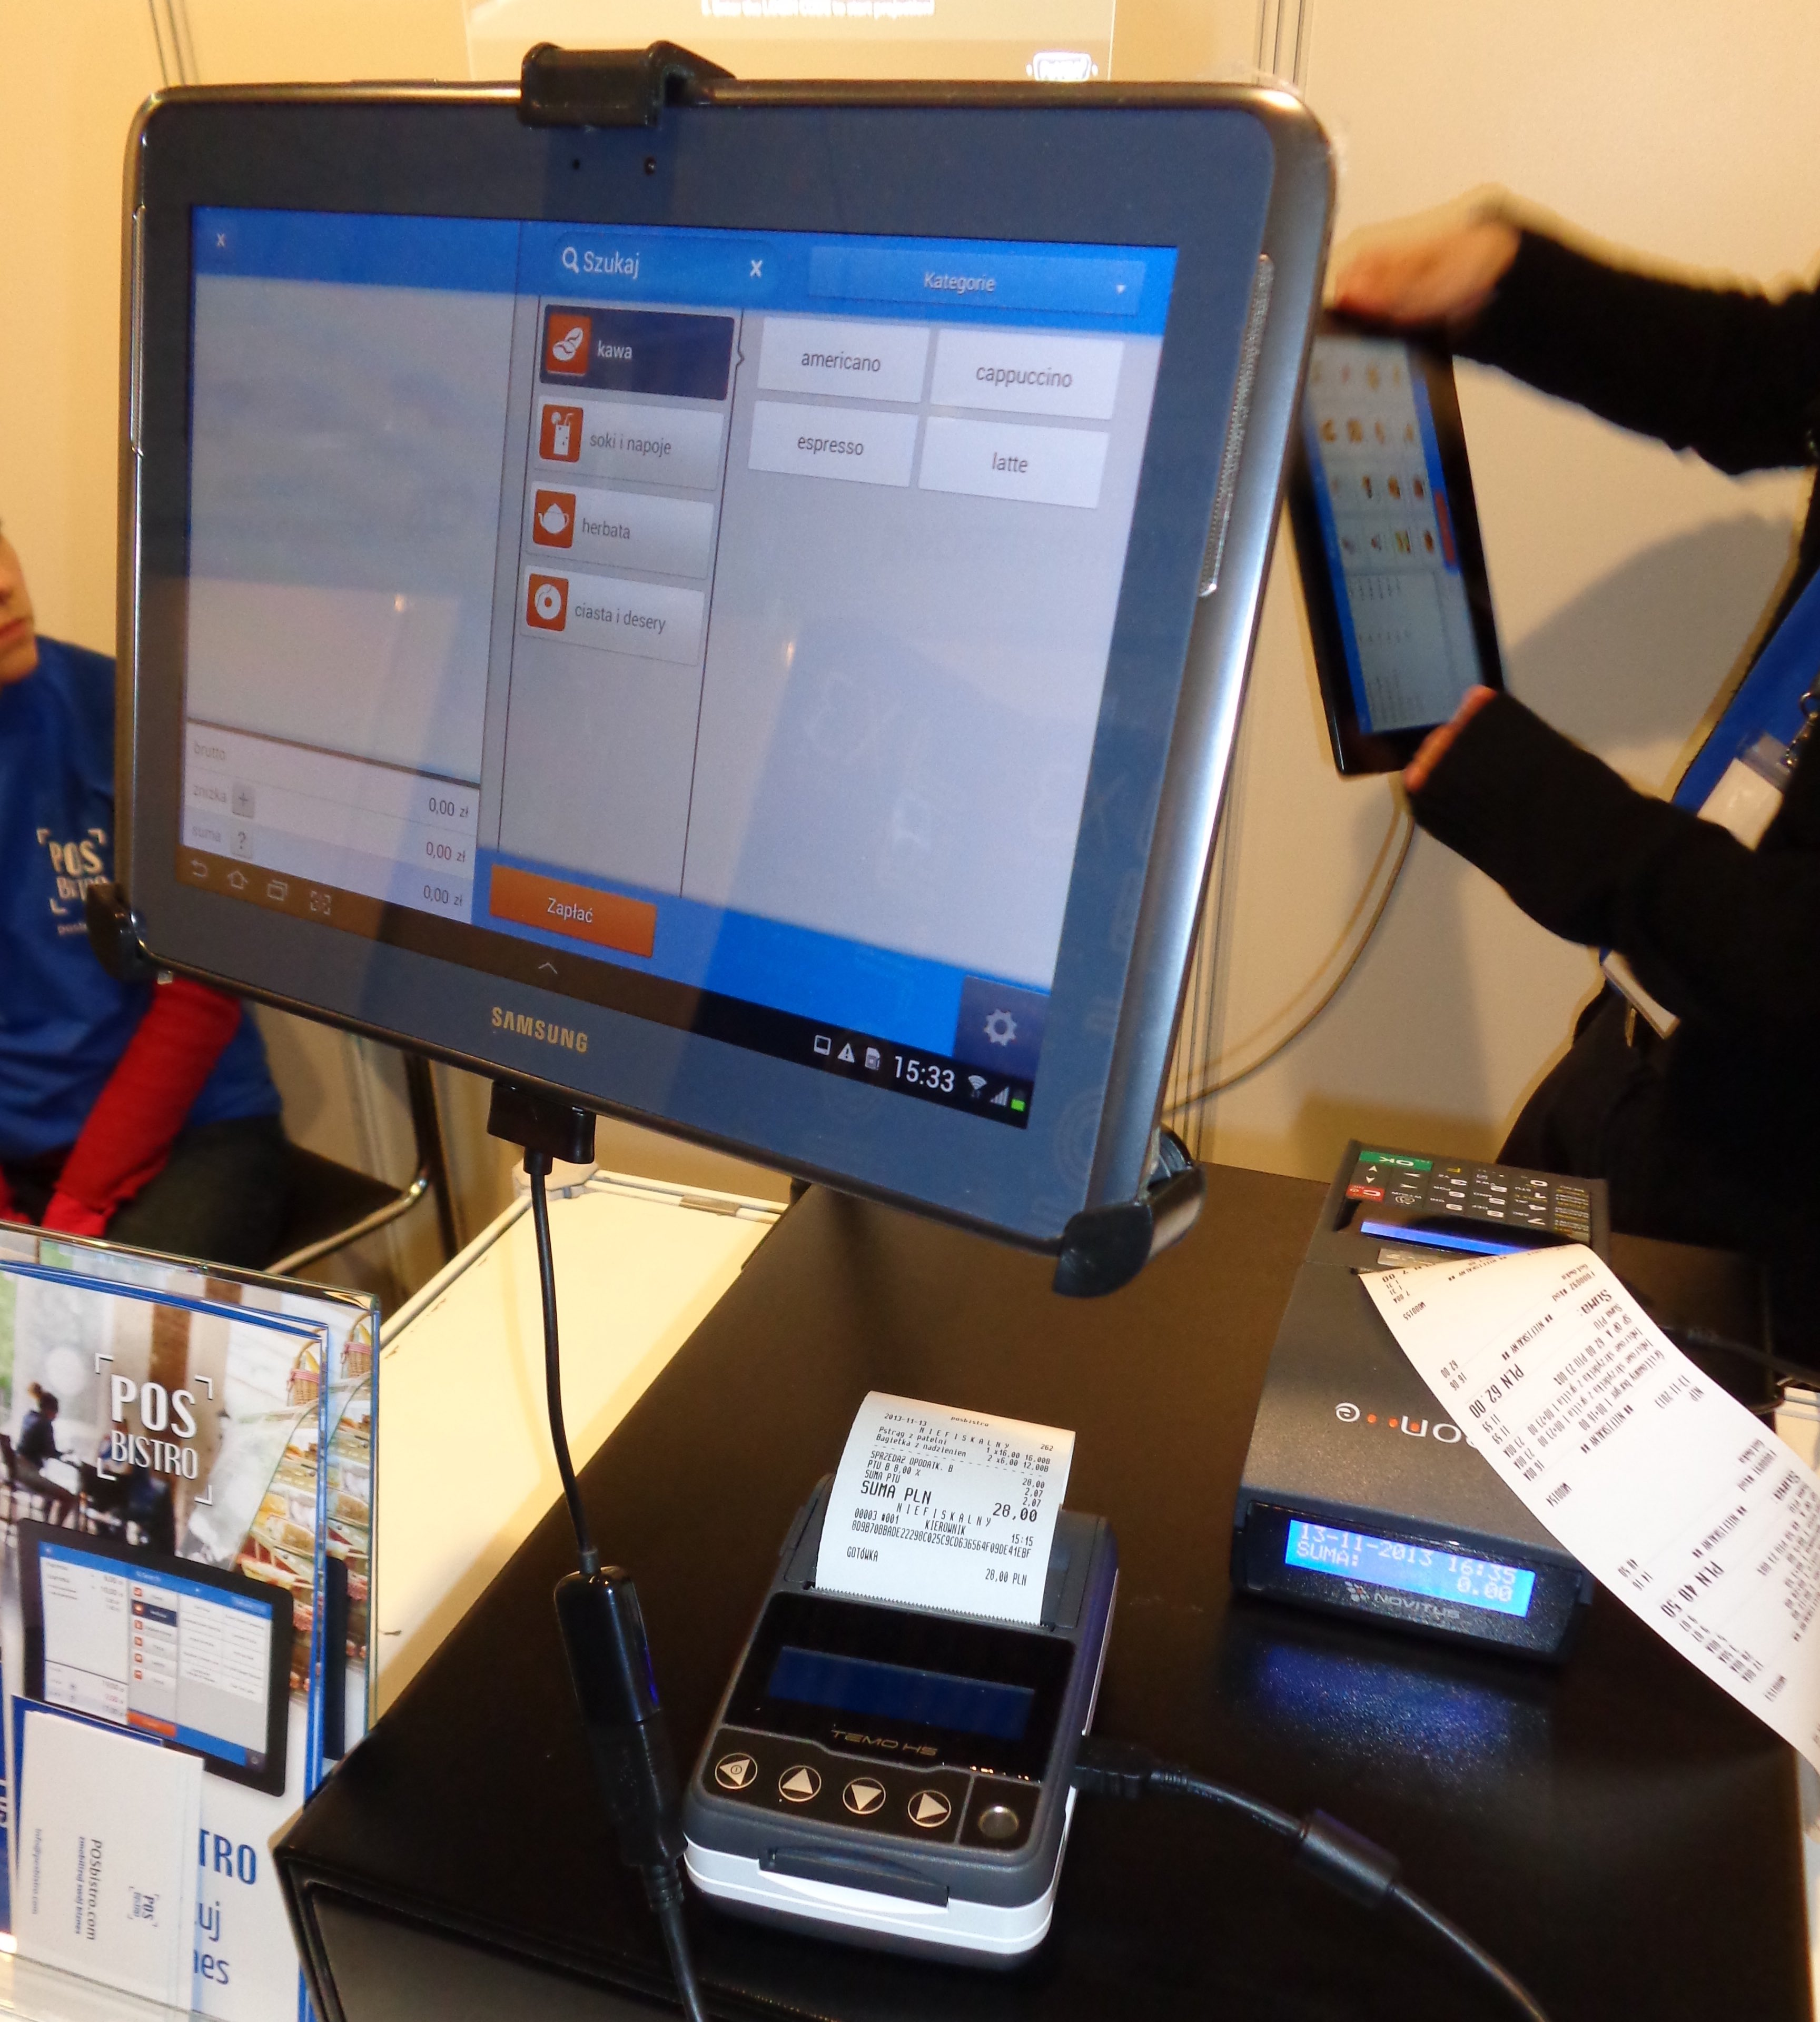
\includegraphics[width=0.9\textwidth]{figs/POS.jpg}
        \caption{\textbf{Existing Devices:} Easily deployed immediately but expensive to deploy to new places. They can also be unreliable when unattended.}
        \footnotetext{wikimedia commons © Travelarz CC-ASA 3.0}
    \end{subfigure}
    ~
    \begin{subfigure}[t]{0.3\textwidth}
        \centering
        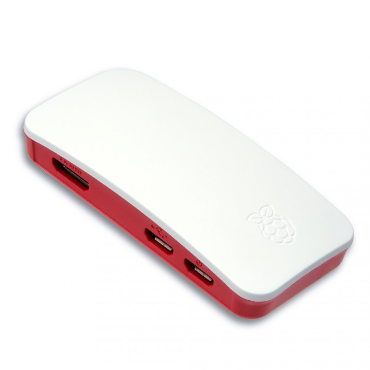
\includegraphics[width=0.9\textwidth]{figs/RaspberryPi.png}
        \caption{\textbf{Dedicated Devices:} Cheap and reliable. They will require new development and can be tricky to place correctly.}
    \end{subfigure}
    ~
    \begin{subfigure}[t]{0.3\textwidth}
        \centering
        
\includegraphics[width=0.9\textwidth]{figs/physicalRPI.pdf}
        \caption{\textbf{No Device:} Allows those without the app or even a mobile device to participate. They may be easier to re-identify and require manual effort from users to check.}
    \end{subfigure}
    \caption{Lighthouses can be deployed using a number of different devices with varying trade-offs. Each of these examples is feasible to deploy in the near future.}
    \label{fig:lighthouseDevices}
\end{figure}

\subsection{What Do We Get From Lighthouses?}
Figure \ref{fig:lighthouseExample} walks through an example of how lighthouses could work in a typical case. Let's explore some of these benefits in more detail.
\begin{figure}
    \centering
    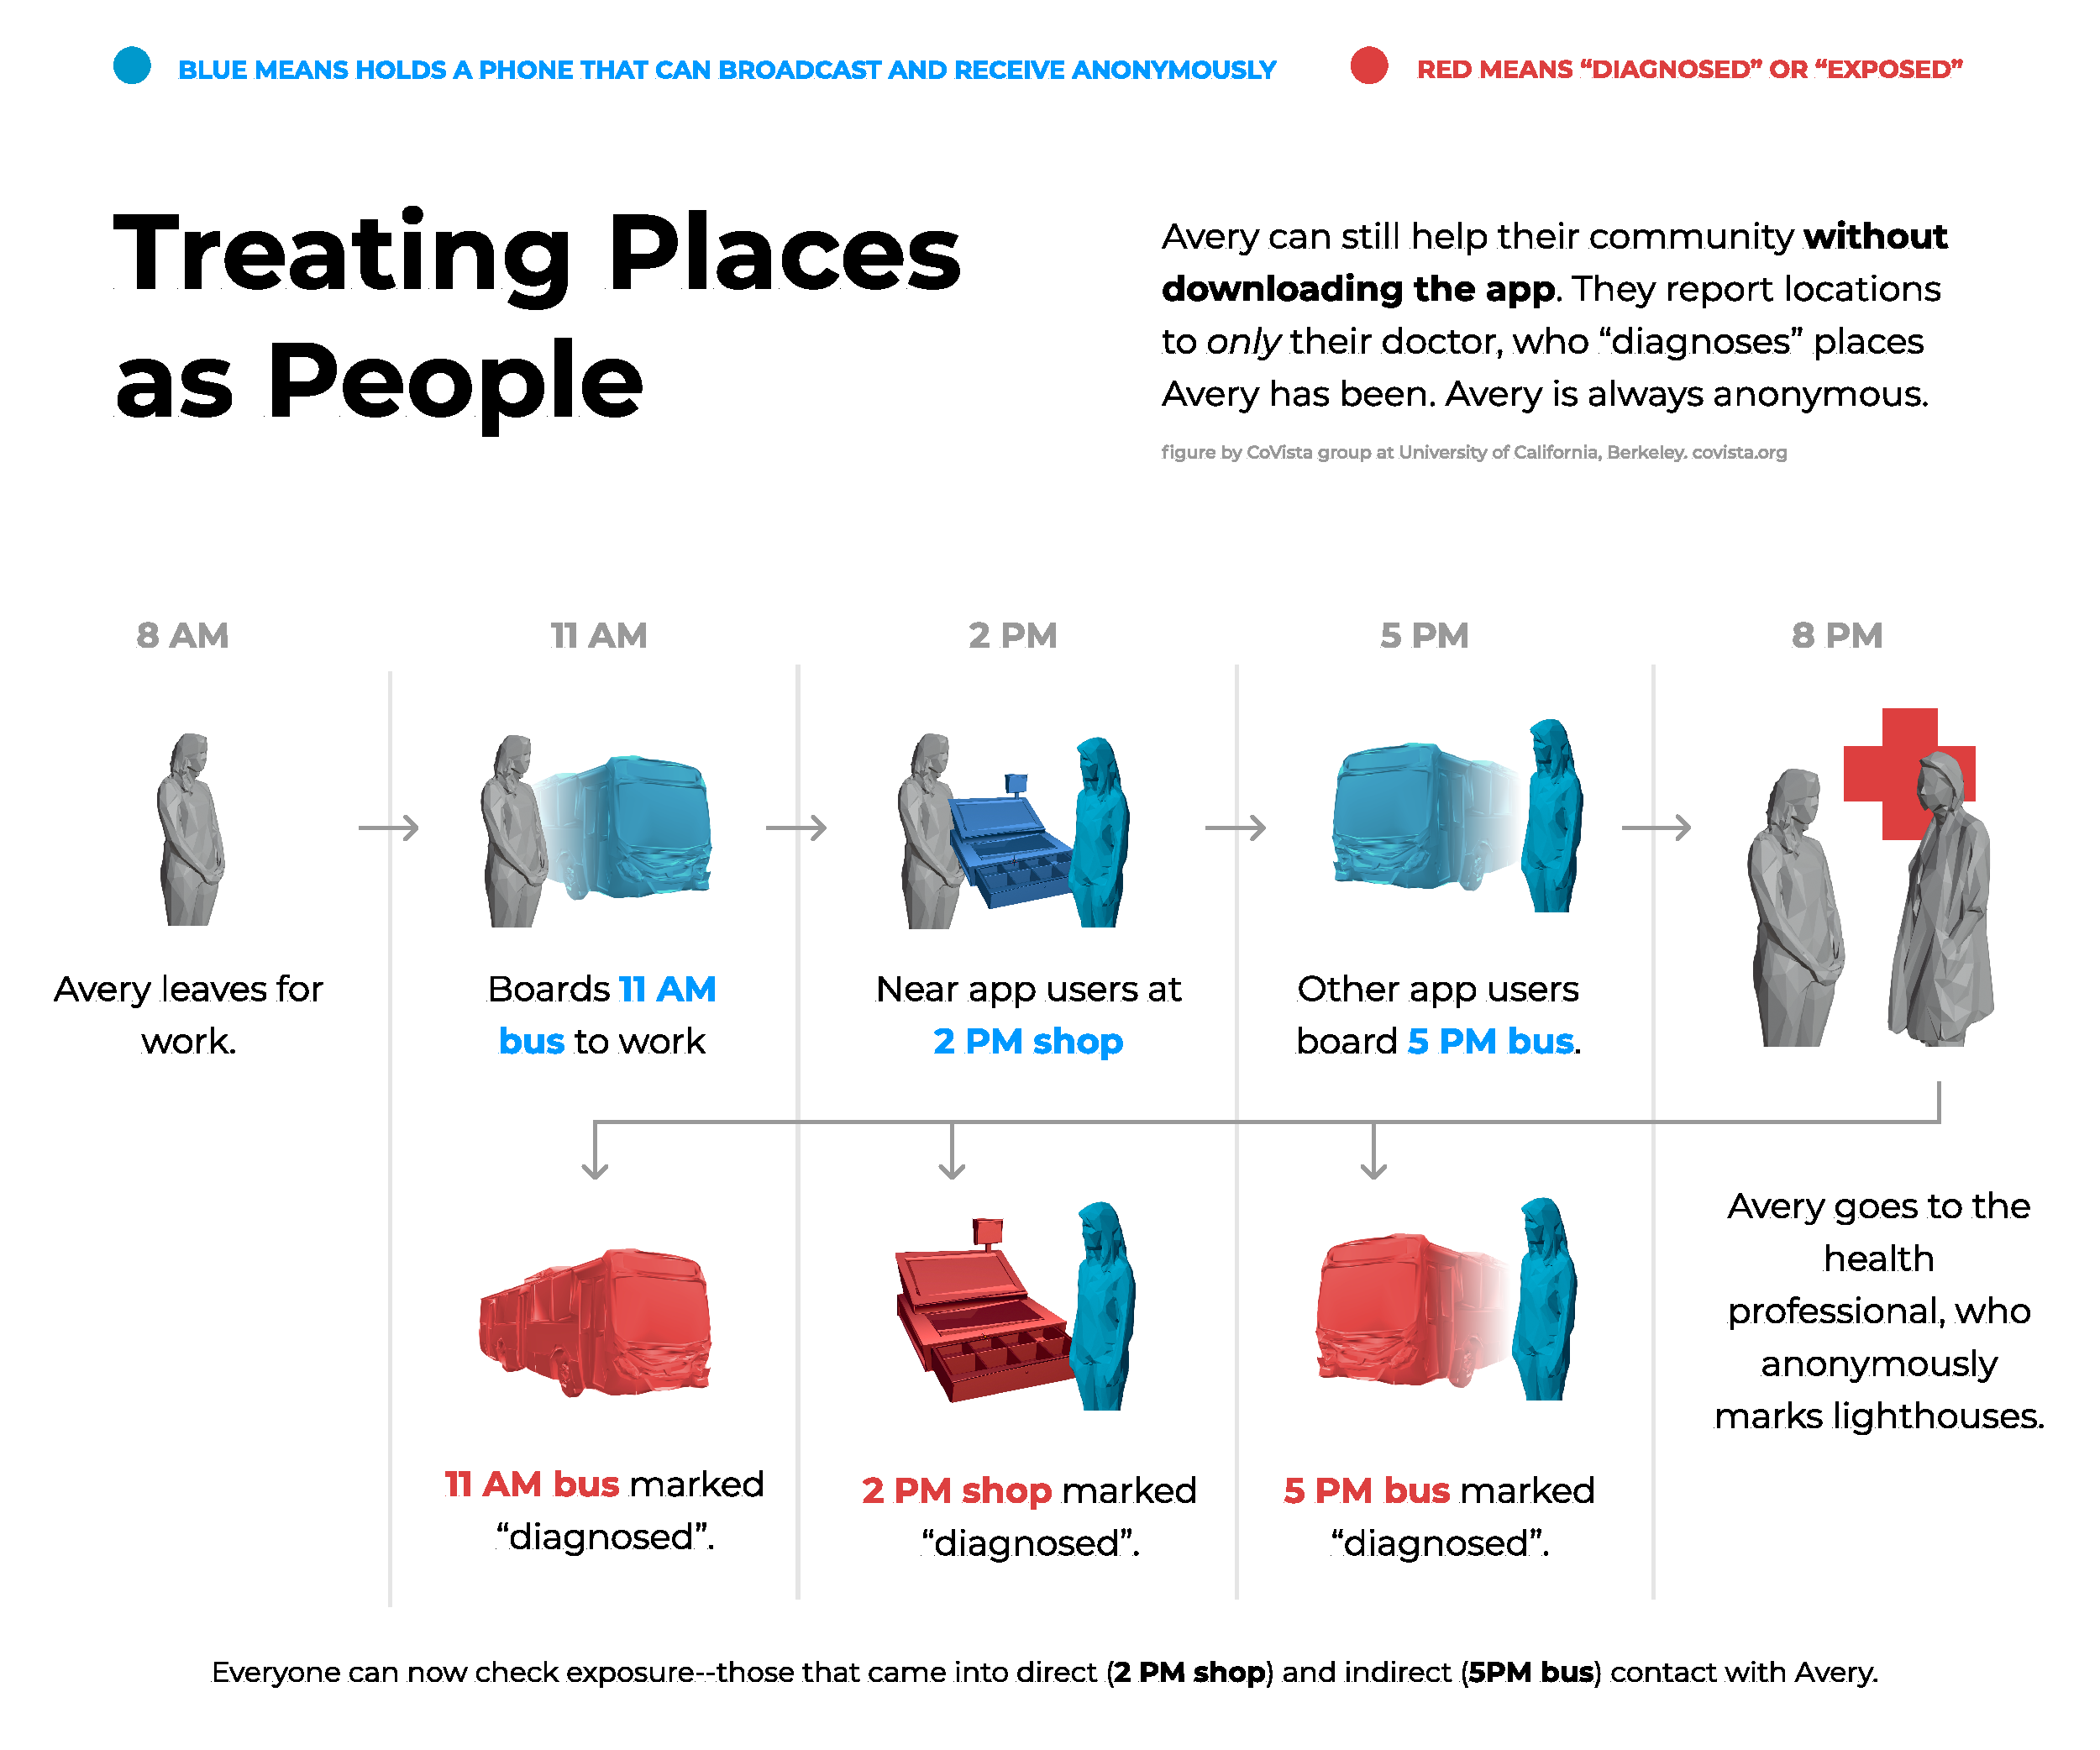
\includegraphics[width=\textwidth]{figs/how_lighthouse_works.pdf}
    \caption{An example scenario of an affected individual (Avery) and a stranger (Bernie) that may have been exposed. Even if Avery is not an app user, the doctor can still notify the shop and bus of their exposure; lighthouses \textbf{connect manual and mobile contact tracing}. Lighthouses \textbf{bridge place and mobile} by allowing the bus and shop to notice their exposure and mark themselves as exposed, even if Avery did not remember visiting them. They also \textbf{enabled less direct forms of exposure} by notifying Bernie of their potential exposure, even though they were not on the bus at the same time as Avery. Finally, lighthouses offer places benefits \textbf{beyond the standard mobile contact tracing}. They can now track how often they are exposed, at what times, and even in which section within them (if they have multiple lighthouses installed).}
    \label{fig:lighthouseExample}
\end{figure}

\shankari{In Fig.~\ref{fig:lighthouseExample}, Avery needs to be diagnosed COVID+ when they go to the health professional. Small change but it needs to happen in Figma}

\shankari{We have generally been using gender-neutral names - Avery and Jordan. Bernie reads as male to me. Use Jordan again?}

\subsubsection{Bridging Place and Mobile}
The contact tracing lighthouse empowers stewards of public spaces (e.g., shop owners, school administrators) to collaborate with public health authorities to help mitigate the spread of disease without jeopardizing the privacy of patrons or the reputation of the public spaces. When an individual is tested and confirmed, the manual contact tracing interview process begins. One of the first questions asked is “Can you recall where you have been that might have exposed others?”. A place, unlike an individual, has a large set of explicit relationships with its institutional environment - business license, health department approvals, chamber of commerce, etc. The interview process routinely seeks to gather information about places. But often there is little the place can do to help. With its lighthouse, it has a very simple way to provide assistance without undue impact on its reputation. Just like a person, it can check its own potential exposures. And, like a person, it can anonymously publish its own random numbers as COVID positive so that people can use them for detecting their exposure risk. This is especially useful if the individual who tested positive was not using an app that broadcasts their own sequence of random numbers. Unlike a person’s phone, stationary lighthouses can be carefully positioned to avoid issues like weak or unreliable broadcast that mobile phones can face. Finally, the public place may also take other measures in assisting its local health authority in detecting hot spots, such as informing them of the exposure risk that it observes.

\subsubsection{Indirect Transmission}
The lighthouse can be used to address forms of indirect transmission that are not captured in the existing privacy-sensitive mobile contact tracing efforts. If a COVID-positive individual enters a bus and touches or sneezes on several surfaces they could potentially infect others over the next several hours, long after they have left the bus. Air conditioning systems have also been implicated in spreading the virus over large distances~\cite{hvacTransmission}. Existing wireless protocols will fail to capture these forms of transmission since they rely on close, contemporaneous radio proximity with the positive individual. However, with the introduction of the lighthouse, the bus or restaurant can automatically determine that it was exposed and choose to anonymously publish its own random number sequence.

\subsubsection{Beyond Mobile Contact Tracing}
Finally, the lighthouse can also extend the privacy-sensitive mobile contact tracing protocol beyond the smartphone. Places provide channels of communication to individuals that complement smartphones. Simple lighthouse codes might be included on printed receipts or handed to customers. A person without contact tracing on their phone might use such code to manually perform the exposure checks that are automated by the apps. For example, they could enter such codes that they have received into a public website to determine their exposure risk.

\subsection{Lighthouse Privacy}
There are legitimate privacy interests for places, as there are for people. 
Businesses may fear irrational boycotts or loss of reputation, and there are risks of perpetuating prejudice or stigma against neighborhoods or ethnic groups (already a growing problem \cite{asianDiscrimination}). The good news is that lighthouses inherit the privacy protecting characteristics of the AGEN protocol. In their simplest form, they are phones running ordinary apps, different only because they live in a fixed place rather than in purse or pocket.

Lighthouses can complement manual contact tracing by offering greater confidentiality in situations where people cross paths in stigmatized locations. For example, investigators following up on a recent case cluster associated with nightclubs in Korea catering to the LGBTQ community have struggled to contact attendees who are afraid of being “outed” or facing discrimination \cite{koreaClub}. Lighthouses can fill such gaps without requiring or relying on anyone, even an affected person, to disclose their location history.

A potential concern about lighthouses is that internal state, if combined and aggregated, could be used to undermine some of the privacy guarantees of AGEN. 
Indeed, with a sufficiently large deployment of lighthouses and centralized collection of recieved RPIs, it would be possible to resolve the locations of all the COVID positive individuals.
We therefore stress that each lighthouse must follow the existing decentralized protocol for risk assessment in which only risk is aggregated and not the underlying RPIs.  

To address some of these security concerns, it is possible to deploy \textbf{transmit only} (passive) lighthouses which could be used to anonymously notify others of exposure without listening for RPIs.  
This eliminates the risk of resolving COVID positive individuals locations but also limits visibility into where the disease is spreading.  




\section{Covid Commons: Unified Contact Tracing With Many Apps}
\label{sec:commons}

% \gabe{this "intro" covers background that should hopefully be established by this point in the paper}

Standardizing on an exposure notification protocol such as AGEN is crucial to achieving the critical mass of participation required to make such an approach effective (estimated to be at least 80\% for a city of 1 million individuals~\cite{hinch2020effective}) and privacy preserving.
Apple and Google, as producers of the two dominant smartphone OSes, are uniquely positioned to bring these capabilities to nearly every smartphone and have engineered the AGEN protocol to that end.
Providing an implementation of the protocol through an OS upgrade would eliminate the fragmentation of the protocol preventing sufficient adoption.
However, standardizing the proximity detection protocol is just part of the solution.

Due to concerns over potential misuse of the capabilities of the proximity detection protocol and location tracking features of modern smartphones, Apple and Google have announced that access to the SDK for AGEN to ``public health agencies"~\cite{agen_pha_announce}.
The realization of this policy has evolved to essentially mean ``one app per state."
Centralizing the apps around state governments means that tracing efforts are not limited to local jurisdictional boundaries. 
However, the public health authorities responsible for testing and tracing often operate at a more local level~\cite{bay_area_testing, local_testing_sites}.

% despite the decentralized nature of the protocol represents the tension between the centralized, location-based manual contact tracing methods traditionally used by governments and public health agencies and the decentralized and privacy-preserving methods developed in academia and industry.

% \gabe{what terminology are we using throughout the paper? exposure/diagnosis keys, etc}
% \joey{We need to udpate the background section to have all of our terminology.}
The fundamental issue with this policy is a failure to distinguish between ownership of the required repository of ``diagnosis keys'' and the applications that produce and utilize them.
The repository contains keys that correspond to times when diagnosed individuals may have interacted with others and must therefore be public-facing so that individuals, via AGEN-compatible apps, can download the keys and determine their own exposure risk.
The keys uploaded to the repository must be limited to those that have been authorized by a public health authority through some testing and interview process.
In the U.S., public health measures such as contact tracing and case reporting are carried out at a county or city level through individually executed processes, in coordination with state and national law and policy.
However, health authorities do not generally have the technical, human or financial resources to produce the required app and also stand up and maintain such a public-facing data service.
This is even less tenable during a pandemic, when such resources are already strained.
Who, then, manages the AGEN backend needed to share Report Keys?

The worst-case scenario is for the repositories to emerge as fragmented silos of diagnosis keys.
In the midst of the custody battle over administration of the emerging technical approaches to the contact tracing problem, it is important to remember that exposure does not respect administrative boundaries.
Regardless of how the repository is established, it is essential that exposure notification can be transmitted across backends and across apps.
Indeed, there are already efforts to combine contact tracing efforts and data across the administrative boundaries established by industry's policy around AGEN~\cite{tri_state_coalition}.

\subsection{A Path to Nation-scale Data}

A solution to this issue is the creation of a privacy-preserving data exchange shared and accessible across apps and administrative boundaries --- a Commons.
Different public health authorities could cooperatively contribute to the Commons and individuals across many jurisdictions would access it through their apps.
Such a Commons might operate at the scale of one per nation, or it might be regional with some form of federation to share keys and exposure information across individual instances.
The Commons may be hosted and maintained by governmental authorities, foundations or other appropriate institutional entities.

The Commons requires no change to the EN protocols.
Each individual participates in the proximity detection using daily TEKs and the RPIs generated from them without change.
With no other information leaving the phone, the app on an indivual phone downloads the diagnosis keys and presents them to the SDK to obtain exposure risk scores.
The difference is that those diagnosis keys are not \emph{a priori} limited to the ones produced by users of the same app.
Just as in the current decentralized protocol, an individual who tests positive --- i.e. a confirmed case --- and participates in contact tracing with a specific public health authority is asked to voluntarily submit their TEKs for the past period over which they are likely to have been contagious.
The AGEN protocol does not stipulate how that request is formulated or how that submission is performed, but the introduction of the Commons allows us to answer that question precisely.

\subsection{The PHA Experience: Federating Access to the Commons}

A Commons is utilized by a well-defined set of public health authorities that are registered with it.
Professionals at PHAs can authenticate to and access the Commons using well-established authentication techniques such as LDAP and OAuth.
As part of requesting a patient to submit their diagnosis keys to the Commons, the professional requests a one-time authorization (OTA) from the Commons.
The OTA authorizes the upload of TEKs corresponding to the extent of time during which the patient is likely to have been contagious; this will involve some days prior to the diagnosis and extend to several days or weeks following.
The OTA is provided to the patient to authorize the submission of their keys to the Commons; the upload is opt-in, as under the usual AGEN protocol.

Because the OTA corresponds to a single interaction between a healthcare professional and a patient, it is a natural key on which helpful metadata can be associated.
The authorizing PHA may want their identity to be associated with the submitted diagnosis keys so that the provenance of the diagnosis is preserved.
This identity, realized by the TLS public key of the PHA, can be associated with generated OTAs in the Commons.
This provides no more information than having each PHA host their own exposure key store, as currently envisioned.
As we will discuss below, the PHA identity can also be used to filter which diagnosis keys are considered in the matching process on an individual's phone.

The OTA itself is also a useful piece of metadata when associated with the uploaded keys in the Commons.
The authorizing professional will likely want to be able to determine whether the patient has in fact contributed their keys as requested to determine if follow-up is necessary.
Associating the OTA with the uploaded keys places no new information in the Commons: the professional knows what they know about those they interview and they know what authorizations they have requested.
Each such confirmed case can be expected to have generated some authorization request, but that information, along with all other aspects of the contact tracing process, is under the purview of the PHA.
Counts of confirmed cases and other aggregate information are already regularly reported to the public.
% They report counts of confirmed cases and various other information to the public.

The Commons is able to provide this functionality despite no patient data --- indeed, no health or medical data of any kind --- ever being entered into the Commons.
The Commons also takes no position on which parts of the contact tracing process are automated and which are manual.
It integrates cleanly with the existing processes established by PHAs for interviewing patients, deciding which diagnosis keys are appropiate to share, and so on.
The Commons merely provides a means of carrying out the result of these decisions in a way that does not require individuals to be using the same phone app.

\subsection{The User Experience: Federating Downloads from the Commons}

\gabe{How much do we want to say here?}

The current draft of the AGEN protocol says very little about how exposure notification information will be transmitted or relayed among the different instances of the diagnosis key repository.
A unified Commons immediately addresses this issue --- all diagnosis keys are uploaded and downloaded from the shared repository.
However, under a federated regime, it is necessary to address how exposure notification and uploaded keys can be routed across instances of the Commons.

Consider a scenario where an individual is diagnosed by one PHA but may travel or may have traveled to regions covered by different PHAs.
Individuals in those other regions should be able to obtain the TEKs for the diagnosed individual, even though the diagnosis was performed by a remote PHA.
There are two complementary approaches.

The first approach proactively forwards diagnosis keys to relevant PHAs.
A PHA professional can ``tag'' a requested OTA with public keys or other metadata identifying relevant remote PHAs, using information acquired as part of the interaction with the individual.
The process of uploading diagnosis keys authorized by that OTA to the Commons can then incorporate a simple forwarding mechanism that replicates those keys to the federated instances of the Commons managed by those other PHAs.
This can be performed by the Commons itself, or it may be performed on an opt-in basis by the individual.

Under the second approach, individuals may proactively request diagnosis key downloads from federated instances of the Commons they are interested in.
An individual may subscribe to diagnosis key downloads for Commons covering regions the individual has travelled to or will travel to.
Additionally, an individual may subscribe to Commons for surrounding regions.

Regardless of whether the Commons is realized as an administratively centralized server or a federated mesh, the Commons must provide some mechanism for filtering or scoping the download of diagnosis keys onto an individual's device.
The number of keys downloaded from the Commons will grow with the adoption of AGEN-based apps, improvements in testing, and the spread of COVID-19.
Without the ability to filter the set of keys down to a reasonable and relevant set that is still large enough to maintain the privacy-preserving properties of AGEN, the bandwidth requirements and compute requirements (for deriving the thousands of RPIs used for the matching process) may grow to be untenable.
\joey{Can we do a small back of the envelope calculation here.}
\gabe{in progress}

\subsection{Extending the Commons}

Once this basic separation of key repository has been established, along with the method for authorizing submissions and routing them to queries, it becomes possible to meaningfully entertain the question of including earlier stages. 
Especially with testing being scarce, confirmation occurs late and involves the contact tracing processes of public health authorities.
Prior to that stage, we have Probable Covid (where a diagnosis has been performed based on defined symptom criteria), preceded by Suspected Covid, and often preceded by individual state of concern. 
Associated with each stage is a process, an (increasingly large) set of principals who might authorize a submission, and a reduced significance in conveying exposure.
For example, the physician or health service making a Probable Covid diagnosis (and typically also authorizing testing) would be the natural principal to authorize the individual to submit “Probable Keys”. 
The privacy-sensitive protocol could access these, as well as the “Confirmed Keys” referred to as Diagnosis Keys in the EN protocol. 
The protocol permits the distinction to be reflected in metadata carried along with the keys. 
Thus they might factor in, perhaps with lesser weight, into the risk score.

% \begin{outline}
% \0 Establish the issue:
%     \1 traditional contact tracing measures require location, invade privacy
%         \2 emergence of PS-MCT protocols
%     \1 standardization of interoperable proximity detection protocol (AGEN) is vital to achieving critical mass of participation
%         \2 need to avoid fragmentation of protocol
%         \2 estimated to be at least 80\% in city of 1 million~\cite{hinch2020effective}
%     \1 Apple/Google in unique position to bring PS-MCT capabilities to nearly every smartphone through OS upgrade
%         \2 expose capabilities through SDK
%         \2 requires a public facing data service to act as broadcast medium
%     \1 2 main concerns w.r.t. AGEN protocol + SDK:
%         \2 misuse of PS-MCT capabilities and information -- leads to limiting release of SDK to public health authorities
%         \2 fragmentation of application -- only allow one contact tracing app per nation or per region
%         \2 centralization of applications (1 per nation), despite decentralized protocol
%    \1 fundamental issue is failure to distinguish between the repo of exposure keys and the the apps that produce/utilize them
%        \2 in US, public health measures such as contact tracing and case reporting are carried out at county or city level in coordination with state and national law and policy
%        \2 health authorities do not have technical, human or financial resources to produce and App and stand up/maintain a public facing data service
%        \2 exposure does not respect administrative boundaries
%            \3 regardless of how repo is established, must be able to transmit exposure notification across backends and across apps
%            \3 tri-state contact tracing coalition (new york, new jersey, connecticut)
%        \2 worst-case scenario is fragmented silos of exposure keys
% \0 establish the solution
%     \1 a Covid Commons -- exposure key database that PHAs cooperatively contribute to and individuals may access
%         \2 can operate at scale of one per nation
%         \2 can operate at smaller scale with some form of federation
%         \2 maintained by govt authority, foundation, institutional entity
% \0 Commons operation
%     \1 how does Commons interact w/ existing PS-MCT protocols
%         \2 the 'commons' fulfills the role of the 'server' in the AGEN protocol
%         \2 upload exposure keys, subject to some authorization from PHA -- one-time auth key
%     \1 how to federate
%         \2 tag auth keys during interaction w/ PHA
%         \2 individual subscribes to (local) PHA, plus other PHAs of interest
% \end{outline}


% However, interoperability of the protocol is only part of the story.


\if 0
\joey{The following is an overview from the position piece here
\url{https://docs.google.com/document/d/1e4_mH7MMYO3bad9BoknrRlWR4jOcKNOFV8UyYLU5kPA/edit}}

Apple/Google Position: An essential part of the companies’ position is to make this basic building block available on every phone and interoperable with all other phones regardless of the manufacturer, operating system, or choice of contact tracing App.
This approach is critical to achieving the adoption needed for these techniques to work.
Apple and Google are not building Apps themselves, instead they have opted to provide access to the APIs exclusively to national public health authorities and their software developers.
The emphasis on directly engaging national public health authorities, rather than local authorities or private App developers, helps to avoid fragmentation of tracing efforts across local governments or Apps.
If the anonymous publication of infected keys is only visible to other users of the same App and in the same region, it would not be possible to identify exposures to users who may have traveled from other regions or chose to install a competing App.

Resolution - Commons: The critical point that Apple and Google missed is that the repository of infected keys needs to be provided in a common, interoperable manner just as does the proximity detection, independent of which App publishes the keys, which health authority handles the contact tracing of the confirmed case, which App accesses the published keys to determine an individual’s risk score, and which public health authorities serves that individual.
Rather than “one app per nation”, a more effective position would be “one Temporary Exposure Key commons per nation”.  This would allow societal structures, rather than corporate policy, to determine how their App ecosystem should evolve.
It is very likely that participation will be greatest if the Apps are available through organizations that individuals trust.  It might be on a city or county basis, a tribal organization, or a community health service.
Such a Covid Commons fits naturally in the privacy-sensitive protocols that have been developed.
When an individual tests positive, they conventionally engage in a contact tracing interview with a public health professional from an established organization, recognized by the Commons.
As part of that interview process, the professional requests a one-time authorization for a set of keys to be contributed by the individual and gives that authorization code to them to enter into their app.
On an opt-in basis, the key set is uploaded.
In this manner, the public health professionals serve to protect the integrity of the information in the Commons without exposing any patient data or medical data.
Their actions are quite similar to publishing counts of cases and demographic information, such as they do today.
And, much as how that statistical data is aggregated today, the Commons provides a means of publication without a complex web of data sharing agreements.
It might be hosted by governmental or NGO structures, based on national or regional policy.
A diverse and innovative App ecosystem can grow to meet the needs of individuals and agencies.
\fi

\if 0
\joey{full text from separate blog post}
%% materials copied from here:
%% https://docs.google.com/document/d/1CUhBwzPkc-iTMBRz1g7OSMb10mKL6Eyxu9o2qQS1UT4/edit

For centuries public health efforts have used “contact tracing” to try to understand and contain the spread of epidemics.The diagnosed patient is interviewed to determine where they have been and who they have been with while contagious.
The interviewer attempts to contact the exposed individuals to identify other cases (hopefully early) expanding the trace and learning of hot spots.
In recent years, some governmental organizations have sought to amplify the reach and efficacy of such measures through surveillance means - cell phone locations or contacts, credit card records, video image processing, and such - raising serious civil liberties and individual privacy concerns, whether access to the information is voluntary or not.

To address these concerns a new privacy sensitive alternative has emerged, privacy sensitive mobile contact tracing.
It leverages standard hardware on modern smartphones to identify and anonymously shares notification of such potential exposures.
Each phone generates a random key on a daily basis and, based on that key, produces a sequence of other seemingly random numbers throughout the day.
Alone, this exchange of random numbers reveals no additional information to the owners of each phone.
When a diagnosed person is interviewed, the public health authority can encourage and allow the patient to share the keys for their contagious period.
Others can access these potential exposure keys, without any information leaving their phones, can compare the random numbers they would produce to ones that the phone has heard.
If there is a strong enough match, the potentially exposed person can then seek guidance, reach out to their health service, request testing, or take other appropriate action.
The health authority exposes no patient data and no health or medical data.
In fact they do little more than what they do in reporting statistics on the cases they encounter.
Yet citizens are able to learn of their individual potential exposure risk.

In order for such exposure risk detection to work, not only must the matching operation be robust and meaningful, but a very large fraction of the population must participate.
Its privacy protections are essential to that.
Ordinary citizens should not be faced with the dilemma of having to give out personal information in order to learn of their exposure risk.
Health and governmental organizations should not be faced with compromising patient privacy in conveying risks to the population.
This privacy sensitive approach to exposure notification eliminates both barriers.

In an astonishing step, Apple and Google joined forces to bring the building blocks of privacy sensitive contact tracing to essentially every smartphone with a routine operating system upgrade.
They engaged with the research community to rapidly mature the low level detection mechanism (Bluetooth Low Energy beacons) and to ensure the cryptographic integrity of the privacy mechanisms.
They recognized the separation of the operating system level service, which performs the cryptography, generates and listens to beacons, and translates matches to a risk score, from “the App”, which provides the user experience and connects the use of this technological mechanism with the professional processes of a local health authority.


Unfortunately, the path that industry, governments, and public health authorities are currently pursuing in the use of this promising approach, despite good intentions, may undermine its potential.
Fearing misuse of these capabilities, the companies announced that they would only release the software development kit (SDK) for Exposure Notification to “public health authorities”.
In the United States, public health measures, especially contact tracing and case reporting, are carried out at the County or City level, in coordination with State and National law and policy.
To have each such health authority produce an App, stand up a public facing data service, and support its operation is untenable.
They generally do not have the technical, human or financial resources to do so, even in the best of times, much less during the incredible crush of the pandemic.
But, even if coordinated industry, state, and federal support could overcome those barriers, the worst path is to produce many distinct silos, fragmenting the pool of exposure keys, be that by County, by App, by platform or any other dividing line.
Covid-19 does not conform to such administrative or political boundaries.

The individual public health authorities do each have their own processes, and they are the appropriate ones to authorize individuals to share their keys, but those keys should be held in common where any potentially exposed person can detect the risks, regardless of County of residence.

Concerns about fragmentation may have prompted the companies to take the unprecedented further step, effectively dictating public health policy, of announcing that they will allow only one contact tracing App per nation to be developed or possibly one per region.
(Specifics of what had been expressed in the new reports have now appeared.)
Interestingly, having faced considerable pressure from certain countries pursuing a centralized approach, rather than a decentralized one, the companies have stood very firm on the decentralized approach but then sought to centralize the Apps.

The fundamental problem here is a failure to recognize the critical distinction between the repository of exposure keys and the Apps that produce and utilize them.
We need to avoid fragmentation and misuse of the repository, regardless of the intended coverage and customization of the Apps.
We see this need reflected in the formation of efforts like the Tri-state Contact Tracing coalition (New York, New Jersey, Connecticut).

The alternative approach would be to create a Covid Commons that many public health authorities cooperatively contribute to and that individuals across those jurisdictions access through their Apps.
Such a Commons could well operate at the scale of one per nation.
Or, it might be regional, with some form of federation.
It might be hosted by a governmental authority, a foundation, or other appropriate institutional entity.

The concept of such a Commons requires no change to the PACT protocol or its Exposure Notification realization.
Each individual participates in BLE proximity detection using daily Temporary Exposure Keys (TEKs) and Rolling Proximity Identifier (RPIs) generated from them without change.
With no other information leaving the phone, the App on the individual phone downloads Diagnosis Keys and presents them to the Exposure Notification SDK to obtain exposure risk scores.
The difference is that those Diagnosis Keys are not a priori limited to the ones produced by users of the same App.

Just as in the current decentralized protocol, an individual who tests positive, i.e., a confirmed case, and participates in contact tracing with a specific public health authority is asked, or requested, to submit their TEKs for the past period over which they are likely to have been contagious.

The Exposure Notification protocol does not stipulate how that request is formulated or how that submission is performed.
The introduction of the Covid Commons allows us to answer that question precisely.
A Commons is utilized by a well-defined set of public health authorities that are registered with it.
Using well-established authentication techniques, the professional at such a PHA can authenticate to and access the Commons.
The action that the professional takes is to request a one-time authorization (OTA) as part of handling a confirmed case.
As part of requesting the patient to submit their Diagnosis Keys, the professional provides the OTA to that individual.
The individual accepts the authorization through their App in as part of submitting those keys.

It is likely that the authorizing PHA would want to have their identity (concretely their TLS Public Key) with the submitted Diagnosis Keys.
This provides no more information than having each PHA host their own exposure key store, as currently envisioned.
Such designations might be used in filtering the keys that are considered for matching.

It is also likely that the authorizing professional might want to be able to determine whether their patient has in fact contributed exposure keys as requested, perhaps to follow up if not.
This places no new information in the Commons.
The professional knows what they know about those they interview, they know what authorizations they have requested.
They report counts of confirmed cases and various other information to the public.
Each such confirmed case can be expected to have generated some authorization request, but that information, along with all other aspects of the contact tracing process, is under the purview of the PHA.

No patient data is entered into the commons.
No health or medical data is entered into it.
In fact, the PHA enters no data into the commons.
But they do have a crucial role.
They are who authorizes an individual to enter specific data into it - via their App.
They are who ensures that the Diagnostic Keys used by individuals to assess their own risk have appropriate integrity.

The introduction of the Commons places no position of which parts of the contact tracing process is automated and which are manual.
The PHA has their own processes for interviewing patients, deciding what Diagnostic Keys are appropriate to share, and so on.
The Commons merely provides a means of carrying out the result of their decisions.
They request a one-time authorization for certain days and they provide it to a certain individual.
How they proceed following that action is entirely according to their particular processes.
Separating off this common key store from the App solves the fragmentation problem.
This separation serves much as does separating proximity detection from the App.
Two individuals do not have to be using the same App in order to appropriately convey risk.
The PHA handling the case determines what gets entered into its store, preserving its integrity.
The low-level BLE proximity detection and the high-level exposure store are both infrastructure that enables the Apps.
They allow an ecosystem of potentially distinct Apps to coexist effectively.

Corporations may have many reasons why they might want to limit the number of groups developing upon one of its products, including limited resources.  But these are business concerns, resolvable by business means.  The issues for the rest of society are participation, privacy, and efficacy.  These are the essential basis for determining how the App ecosystem should evolve.

Once the Commons (and the proximity) detection are separated from the App and made interoperable, a strong argument can be made for Apps that are tailored for the community they serve.  This may be the strongest reason for having local health authorities “provide” the App - by which we mean they shape the user experience, not that each PHA becomes an App developer.  But they should be able to skin it, brand it, and tailor it to their processes. Personal privacy is critical for participation, and so is trust.  It is easy to imagine that a person will be more likely to use an App if it is associated with the local entity that is providing testing, support, guidelines, etc.  The entity they trust.  The App can bring value to the individual beyond the detection of risks (which we hope is rare) and submission of keys (if so unfortunate as to be diagnosed positive), it can provide current local information that is useful everyday.  And, if they do experience risk, rather than just a vague score and perhaps a contact of a state or national level service, it can provide specific guidance relevant to the processes of the local public health authority, health services, testing capacities, and so on.  It can be tailored and actionable.

It is useful to look separately at the two kinds of engagements with Exposure Notification.  Take first the case where an individual has been confirmed and is involved in the contact tracing process.  That process is carried out by an organization according to a particular flow.  Does the individual prepare materials in advance of the interview, during or after?  How are questions asked and follow-up performed?  At what points in this process are what sorts of information provided?  If the technology for privacy-sensitive mobile contact tracing is going to improve the efficiency and efficacy of that contact tracing process, it should be responsive to that process, rather than dictate some other process that might seem to fit the technology.  The ability to customize and tailor would seem to be critical to efficacy, as well as participation.

The confirmed case is sourced from a particular institutional authority.  Thus, it is natural for that authority to authorize its inclusion and potentially make an effort to encourage its submission.  And to some extent it reflects where to consider for exposure. Often, confirmed and exposed individuals will be part of the same community and share the institutional authority.  But not entirely.  A person may live in one county but work or go to school in another.  The individual assessing their exposure risk knows where they have been and they might configure their app to include the PHAs for those places.  (Even with very crude location determination, this might be done automatically.) Accessing those is straightforward with a Commons (just a filter) but could be accomplished even with a directory of the many distinct stores (if they all used a standard access method).  But the confirmed individual may have reported in some institutional jurisdiction other than that where the exposure occurred.

Instead, the federation of data may be better driven from the source entity.  In the interview process the health professional obtains knowledge of what areas the confirmed patient has occupied while contagious.  So in requesting the OTA it is natural to provide indication of potentially affected areas, along with the authorized dates of keys.  When the Diagnosis Keys are submitted, they can be included in the exposure requests where there is potential exposure.

Once this basic separation of key repository has been established, along with the method for authorizing submissions and routing them to queries, it becomes possible to meaningfully entertain the question of including earlier stages.  Especially with testing being scarce, confirmation occurs late and involves the contact tracing processes of public health authorities. Prior to that stage, we have Probable Covid (where a diagnosis has been performed based on defined symptom criteria), preceded by Suspected Covid, and often preceded by individual state of concern.  Associated with each stage is a process, an (increasingly large) set of principals who might authorize a submission, and a reduced significance in conveying exposure. For example, the doctor or health service making a Probable Covid diagnosis (and typically also authorizing testing) would be the natural principal to authorize the individual to submit “Probable Keys”.  The privacy-sensitive protocol could access these, as well as the “Confirmed Keys” referred to as Diagnosis Keys in the EN protocol.  The protocol permits the distinction to be reflected in metadata carried along with the keys.  Thus they might factor in, perhaps with lesser weight, into the risk score.
\fi







\vspace{-.5cm}
\section{Conclusion}
\label{sec:conclusion}

Online job platforms are becoming increasingly popular.
They provide an alternative job arrangement that has the potential to dramatically affect the Future of Work. 
An increasing proportion of human workforce will be employed in such platforms.
Hence, it is very important to study the problem of platform design.
In this paper, we have a preliminary attempt at investigating this problem.
We provide a taxonomy of platforms and what are the major missing functionalities for both workers and requesters. 
We also advocate the need for interoperability between platforms.
This allows workers and requesters to move their data between platforms without getting locked into a single platform. 
There are a number of interesting research and policy challenges in achieving the vision of platform interoperability.



% \bibliographystyle{IEEEtran}
% \bibliography{ms}
% \bibliography{submissions/BerkeleyCovista/ms}

% Generated by IEEEtran.bst, version: 1.14 (2015/08/26)
\begin{thebibliography}{10}
\providecommand{\url}[1]{#1}
\csname url@samestyle\endcsname
\providecommand{\newblock}{\relax}
\providecommand{\bibinfo}[2]{#2}
\providecommand{\BIBentrySTDinterwordspacing}{\spaceskip=0pt\relax}
\providecommand{\BIBentryALTinterwordstretchfactor}{4}
\providecommand{\BIBentryALTinterwordspacing}{\spaceskip=\fontdimen2\font plus
\BIBentryALTinterwordstretchfactor\fontdimen3\font minus
  \fontdimen4\font\relax}
\providecommand{\BIBforeignlanguage}[2]{{%
\expandafter\ifx\csname l@#1\endcsname\relax
\typeout{** WARNING: IEEEtran.bst: No hyphenation pattern has been}%
\typeout{** loaded for the language `#1'. Using the pattern for}%
\typeout{** the default language instead.}%
\else
\language=\csname l@#1\endcsname
\fi
#2}}
\providecommand{\BIBdecl}{\relax}
\BIBdecl

\bibitem{agen}
\BIBentryALTinterwordspacing
A.~Inc., \emph{"Apple and Google partner on COVID-19 contact tracing
  technology"}, 10 April 2020 (accessed 25 May 2020). [Online]. Available:
  \url{https://web.archive.org/web/20200410171128/https://www.apple.com/newsroom/2020/04/apple-and-google-partner-on-covid-19-contact-tracing-technology/}
\BIBentrySTDinterwordspacing

\bibitem{pact}
J.~Chan, D.~Foster, S.~Gollakota, E.~Horvitz, J.~Jaeger, S.~Kakade, T.~Kohno,
  J.~Langford, J.~Larson, P.~Sharma, S.~Singanamalla, J.~Sunshine, and
  S.~Tessaro, ``Pact: Privacy sensitive protocols and mechanisms for mobile
  contact tracing,'' 2020.

\bibitem{dp3t}
\BIBentryALTinterwordspacing
C.~e.~a. Troncoso, \emph{Decentralized Privacy-Preserving Proximity Tracing}.
  [Online]. Available:
  \url{https://github.com/DP-3T/documents/blob/master/DP3T%20White%20Paper.pdf}
\BIBentrySTDinterwordspacing

\bibitem{traceTogether20pct}
\BIBentryALTinterwordspacing
\emph{20 April 2020 - One Month On}, 20 April 2020 (Accessed 24 May 2020).
  [Online]. Available:
  \url{https://web.archive.org/web/20200524045214/https://support.tracetogether.gov.sg/hc/en-sg/articles/360046475654-20-April-2020-One-Month-On}
\BIBentrySTDinterwordspacing

\bibitem{hvacTransmission}
J.~Lu, J.~Gu, K.~Li, C.~Xu, W.~Su, and Z.~e.~a. Lai, ``Covid-19 outbreak
  associated with air conditioning in restaurant, guangzhou, china, 2020,''
  \emph{Emerging Infectious Disease}, 2020,
  https://doi.org/10.3201/eid2607.200764.

\bibitem{asianDiscrimination}
\BIBentryALTinterwordspacing
E.~Y.-J. Kang, \emph{Asian Americans Feel The Bite Of Prejudice During The
  COVID-19 Pandemic}, National Public Radio, 31 March 2020 (Accessed 2 April
  2020). [Online]. Available:
  \url{https://web.archive.org/web/20200402203217/https://www.npr.org/local/309/2020/03/31/824397216/asian-americans-feel-the-bite-of-prejudice-during-the-c-o-v-i-d-19-pandemic}
\BIBentrySTDinterwordspacing

\bibitem{koreaClub}
\BIBentryALTinterwordspacing
H.~Shin and J.~Smith, ``South korea scrambles to contain nightclub coronavirus
  outbreak,'' \emph{Reuters}, 2020. [Online]. Available:
  \url{https://www.reuters.com/article/us-health-coronavirus-southkorea/south-korea-scrambles-to-contain-nightclub-coronavirus-outbreak-idUSKBN22N0DA}
\BIBentrySTDinterwordspacing

\bibitem{hinch2020effective}
\BIBentryALTinterwordspacing
R.~Hinch, W.~Probert, A.~Nurtay, M.~Kendall, C.~Wymant, M.~Hall, and C.~Fraser,
  ``Effective configurations of a digital contact tracing app: A report to
  nhsx,'' 2020. [Online]. Available:
  \url{https://github.com/BDI-pathogens/covid-19_instant_tracing/blob/master/Report
  - Effective Configurations of a Digital Contact Tracing App.pdf}
\BIBentrySTDinterwordspacing

\bibitem{agen_pha_announce}
\BIBentryALTinterwordspacing
\emph{Exposure Notification API launches to support public health agencies},
  Apple Incorporated, Google LLC, 20 May 2020 (Accessed 24 May 2020). [Online].
  Available:
  \url{http://web.archive.org/web/20200524152945/https://blog.google/inside-google/company-announcements/apple-google-exposure-notification-api-launches/}
\BIBentrySTDinterwordspacing

\bibitem{bay_area_testing}
\BIBentryALTinterwordspacing
C.~Ho, ``Bay area coronavirus tests: Where can i get one?'' 21 May 2020
  (Accessed 25 May 2020). [Online]. Available:
  \url{http://web.archive.org/web/20200525201614/https://www.sfchronicle.com/health/article/Where-can-I-get-a-coronavirus-test-in-the-Bay-15136054.php}
\BIBentrySTDinterwordspacing

\bibitem{local_testing_sites}
\BIBentryALTinterwordspacing
N.~A. of~County and C.~H. Officials, ``Directory of local health departments,''
  24 May 2020 (Accessed 24 May 2020). [Online]. Available:
  \url{http://web.archive.org/web/20200524090932/https://www.naccho.org/membership/lhd-directory}
\BIBentrySTDinterwordspacing

\bibitem{tri_state_coalition}
\BIBentryALTinterwordspacing
N.~N. York, ``What you need to know about {N}ew {Y}ork’s ‘monumental’
  contact tracing program,'' 22 April 2020 (Accessed 24 May 2020). [Online].
  Available:
  \url{http://web.archive.org/web/20200524162632/https://www.nbcnewyork.com/news/coronavirus/what-you-need-to-know-about-new-yorks-monumental-contact-tracing-program/2385611/}
\BIBentrySTDinterwordspacing

\end{thebibliography}



\end{document}
